\documentclass[table]{beamer}
%%\documentclass[handout]{beamer}

\mode<presentation>
{
  \definecolor{navitialight}{RGB}{126,186,200}
  \definecolor{navitiadark}{RGB}{76,102,114}

  \useoutertheme[subsection=false]{miniframes}
  %%\useoutertheme[footline=authortitle]{miniframes}
  \usecolortheme[named=navitiadark]{structure}
  %%\usecolortheme{dolphin}
  \usecolortheme{orchid}
  \useinnertheme{circles}
  \setbeamerfont{block title}{size=\normalsize}
  \setbeamercovered{transparent}

  %%% le foot pour avoir la numérotation des slides %%%
  \setbeamertemplate{footline}{%
    \leavevmode%
    \hbox{%
      \begin{beamercolorbox}[wd=.5\paperwidth,ht=2.5ex,dp=1.125ex,
        leftskip=.3cm plus1fill,rightskip=.3cm]{author in head/foot}%
        \usebeamerfont{title in head/foot}\insertshorttitle
      \end{beamercolorbox}%
      \begin{beamercolorbox}[wd=.5\paperwidth,ht=2.5ex,dp=1.125ex,
        leftskip=.3cm,rightskip=.3cm plus1fil]{title in head/foot}%
        \usebeamerfont{author in head/foot}\insertshortauthor\hfill
        \insertframenumber/\inserttotalframenumber
      \end{beamercolorbox}%
    }%
    \vskip0pt%
  }

  \setbeamercolor{palette primary}{fg=white,bg=navitiadark}
  \setbeamercolor{palette secondary}{fg=white,bg=navitialight}
  \setbeamercolor{palette tertiary}{fg=white,bg=navitiadark}
  \setbeamercolor{palette quaternary}{fg=white,bg=navitialight}
}

\mode<handout>
{
  \usepackage{pgfpages}
  \pgfpagesuselayout{4 on 1}[a4paper,border shrink=5mm,landscape]
}

\usepackage[utf8]{inputenc}
\usepackage{lmodern}
\usepackage[T1]{fontenc}
\usepackage[english,francais]{babel}
\usepackage{multirow}
\usepackage{hhline}

\newcommand{\nologo}{\setbeamertemplate{logo}{}}

\newenvironment{foreignpar}[1][english]{%
    \em\selectlanguage{#1}%
}{}
\newcommand*{\foreign}[2][english]{%
    \emph{\foreignlanguage{#1}{#2}}%
}

\title[BANO + OSM + Navitia]{BANO + OSM + Navitia = un nouveau géocodeur pour les transports}

\author{Guillaume Pinot \and Noémie Lehuby \and Pascal Rhod}

\institute[Kisio Digital] % (optional, but mostly needed)
{
  Kisio Digital\\
  20 rue Hector Malot\\
  75012 Paris, France}
%% - Use the \inst command only if there are several affiliations.
%% - Keep it simple, no one is interested in your street address.

\date{State of the Map France 2017}
%% - Either use conference name or its abbreviation.
%% - Not really informative to the audience, more for people (including
%%   yourself) who are reading the slides online

%% If you have a file called "university-logo-filename.xxx", where xxx
%% is a graphic format that can be processed by latex or pdflatex,
%% resp., then you can add a logo as follows:
\pgfdeclareimage[width=.2\linewidth]{logo}{images/logo_nio}
\logo{\pgfuseimage{logo}\hspace{.04\linewidth}}


%% Delete this, if you do not want the table of contents to pop up at
%% the beginning of each subsection:
\AtBeginSection[]
{
  \begin{frame}<beamer>
    \frametitle{Table des matières}
    \tableofcontents[currentsection,hideothersubsections]
  \end{frame}
}
\AtBeginSubsection[]
{
  \begin{frame}<beamer>
    \frametitle{Table des matières}
    \tableofcontents[currentsection,subsectionstyle=show/shaded/hide]
  \end{frame}
}


\begin{document}

\begin{frame}
  \titlepage
\end{frame}

\section{Pourquoi?}

\begin{frame}
  \frametitle{navitia}

  \begin{itemize}
  \item le cœur de l'information voyageur de Kisio Digital
  \item une API REST
    \begin{itemize}
    \item calcul d'itinéraire multimodal
    \item fiche horaires
    \item prochains passages
    \item autocompletion et géocodage inverse
    \end{itemize}
  \item disponible via \url{https://navitia.io}, notre service ouvert
  \end{itemize}
\end{frame}

\begin{frame}
  \frametitle{Nouveaux besoins autour du géocodage}

  \begin{itemize}
  \item autocompletion sans pré-filtre géographique (\foreign{coverage} dans Navitia)
  \item autocompletion potentiellement sur le monde
  \item prise en compte de la localisation de l'utilisateur
  \item gestion des zones d'arrêt en fonction des droits de l'utilisateur
  \item séparation en (plus de) microservice
  \end{itemize}
\end{frame}

\begin{frame}
  \frametitle{Et l'existant?}

  \centering\footnotesize
  \begin{tabular}{|c|ccl|}
    \hline
    projet & technologie & fautes & problèmes\\
    \hline
    NAViTiA 1 & custom & phonétique, distance & pas d'évolution\\
    navitia 2 & custom & 3gram & pas de géo, mise à l'échelle\\
    photon & elasticsearch & distance & alimentation OSM seul\\
    addok & redis & phonétique, distance & mémoire, qualité des fautes\\
    \hline
  \end{tabular}
\end{frame}

\section{Les données}

\begin{frame}
  \frametitle{OpenStreetMap: les villes}

  Utilisation des villes, arrondissement, pays... (\foreign{administrative regions}):
  \begin{itemize}
  \item \foreign{level} configurable
  \item utilisation INSEE, code postaux
  \item import des contours géographiques
  \item coordonnées grâce au \foreign{role} \texttt{center} ou au
    barycentre du contour
  \end{itemize}
\end{frame}

\begin{frame}[fragile]
  \frametitle{OpenStreetMap: les POI}

  \begin{itemize}
  \item configuration à la lecture d'OSM
  \item type de POI
  \item si pas de \texttt{name}, utilisation du type de POI
  \item coordonnées en fonction du type de l'objet
  \end{itemize}

  \tiny
\begin{verbatim}
{
  "poi_types": [
    {"id": "amenity:school", "name": "École"},
    {"id": "amenity:bar_tobacco", "name": "Bar-tabac"},
  ],
  "rules": [
    {
      "osm_tags_filters": [{"key": "amenity", "value": "college"}],
      "poi_type_id": "amenity:school"
    },
    {
      "osm_tags_filters": [{"key": "amenity", "value": "university"}],
      "poi_type_id": "amenity:school"
    },
    {
      "osm_tags_filters": [{"key": "amenity", "value": "cafe"}, {"key": "tobacco", "value": "yes"}],
      "poi_type_id": "amenity:bar_tobacco"
    }
  ]
}
\end{verbatim}
\end{frame}

\begin{frame}
  \frametitle{OpenStreetMap: les rues}

  Utilisation des rues:
  \begin{itemize}
  \item regroupement des \foreign{ways} grâce à
    \texttt{associatedStreet} ou par ville
  \item affectation de la ville grâce aux contours géographiques
  \item coordonnées grâce à un point des \foreign{ways}
  \end{itemize}
\end{frame}

\begin{frame}[fragile]
  \frametitle{BANO: les adresses}

  \begin{itemize}
  \item import direct des adresses
  \item rattachement des régions administratives par INSEE et contours
  \end{itemize}

\scriptsize
\begin{verbatim}
751124517P-20,20,Rue Hector Malot,75012,Paris,OSM,48.846781,2.377150
\end{verbatim}

\begin{verbatim}
{
  "house_number": "20",
  "street": {
    "street_name": "Rue Hector Malot",
    "administrative_regions": [
      {"insee": "75112", "level": 9, "name": "Paris", "zip_codes": ["75012"]},
      {"insee": "75056", "level": 8, "name": "Paris", "zip_codes": []}
    ],
  },
  "label": "20 Rue Hector Malot (Paris)",
  "coord": { "lat": 48.846781, "lon": 2.37715 },
  "zip_codes": ["75012"]
}
\end{verbatim}
\end{frame}

\begin{frame}
  \frametitle{GTFS: les zones d'arrêt}

  \begin{block}{Le \foreign{General Transit Feed Specification}
      (GTFS)}
    \begin{itemize}
    \item Standard des données de transport
    \item ensemble de fichier CSV
    \end{itemize}
  \end{block}

  \begin{columns}
    \begin{column}{.65\linewidth}
      \begin{itemize}
      \item import des zones d'arrêt uniquement (\texttt{location\_type=1})
      \item importance par nombre de point d'arrêt
      \item rattachement des régions administratives par contours
      \end{itemize}
    \end{column}
    \begin{column}{.35\linewidth}
      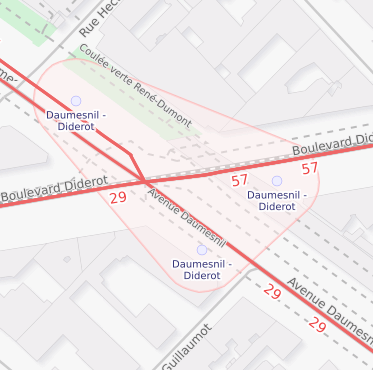
\includegraphics[width=\textwidth]{images/stop-area}
    \end{column}
  \end{columns}

\end{frame}

\section{La recherche}

\begin{frame}
  \frametitle{Autocompletion par type}

  \centering
  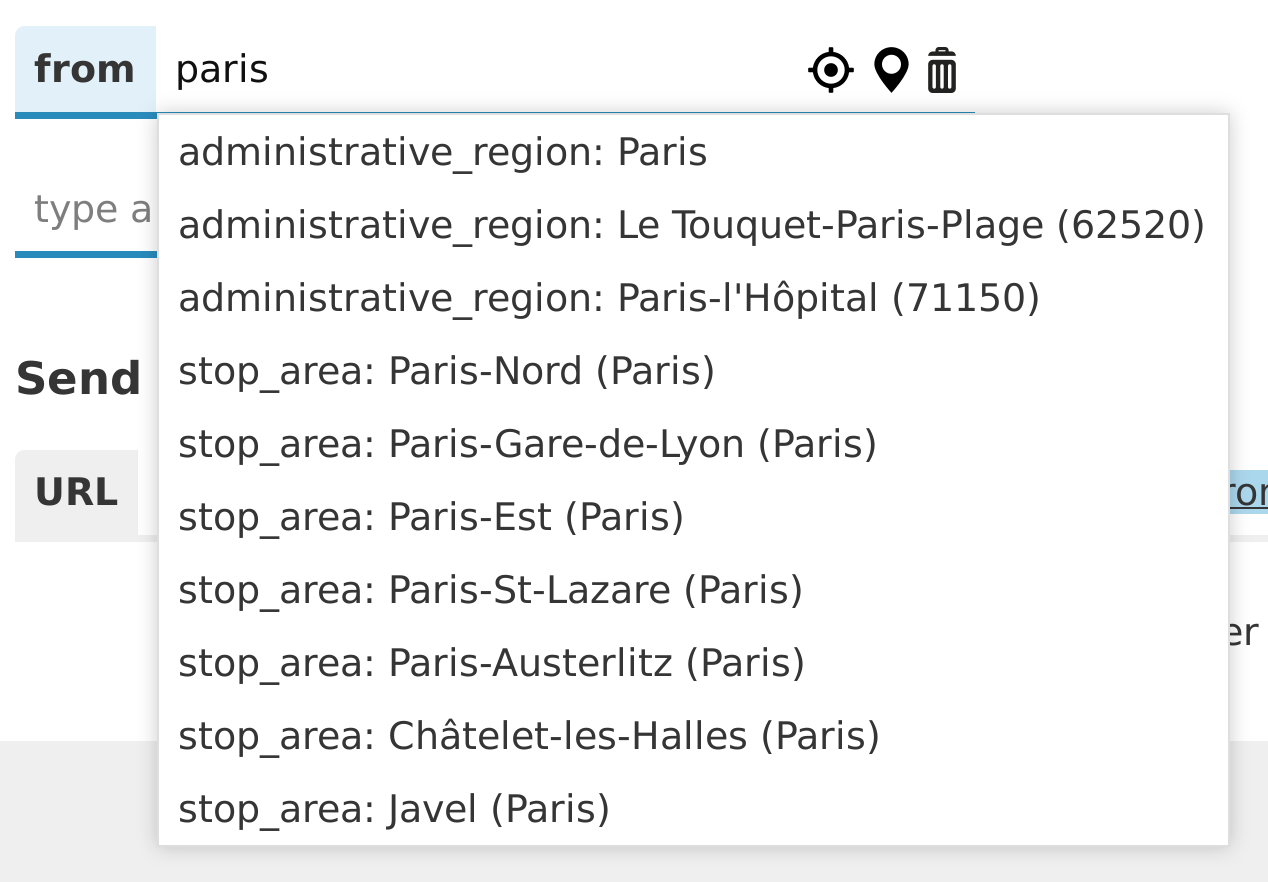
\includegraphics[width=0.7\linewidth]{images/autocomplete-paris}
\end{frame}

\begin{frame}
  \frametitle{Autocompletion tolérante aux fautes}

  \centering
  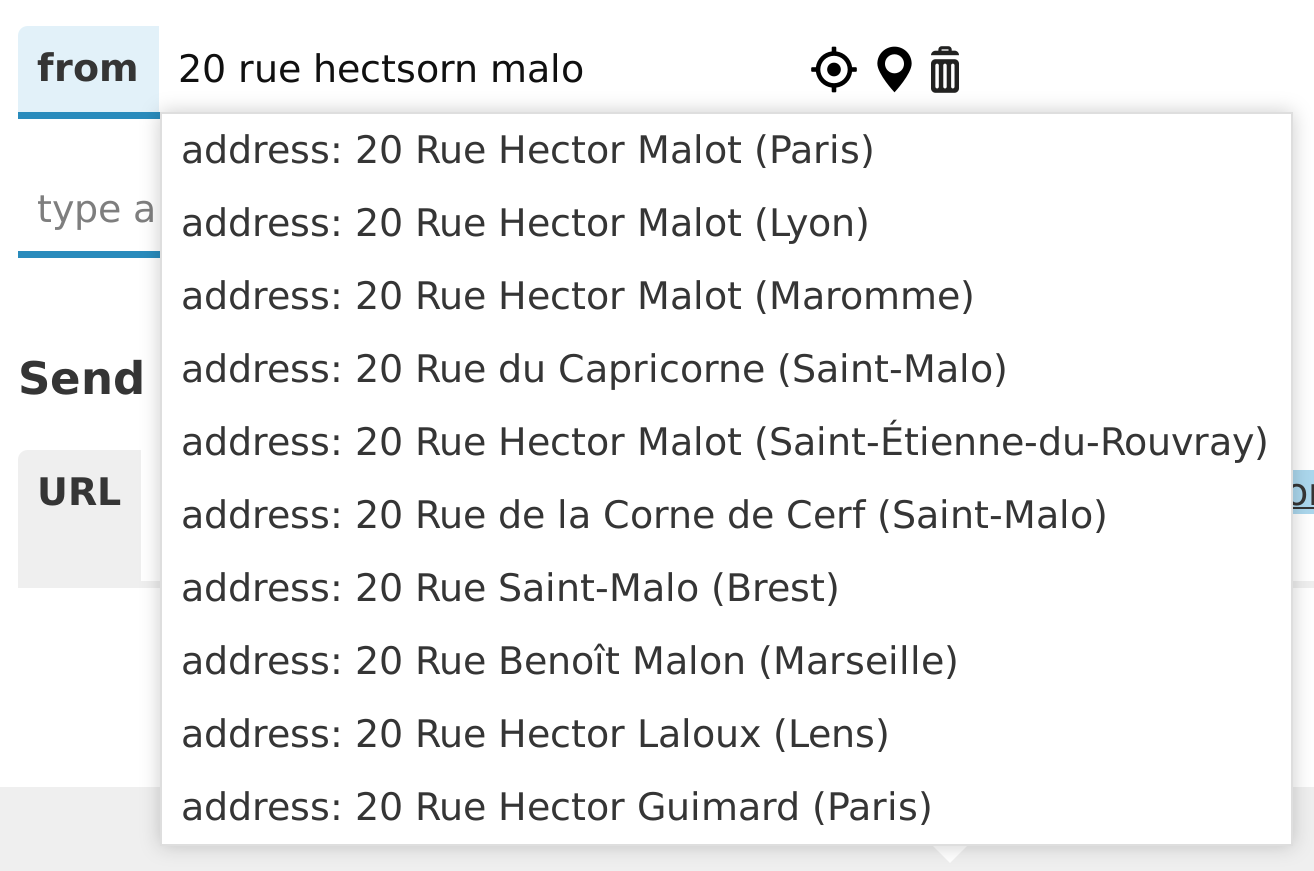
\includegraphics[width=0.7\linewidth]{images/autocomplete-typo}
\end{frame}

\begin{frame}
  \frametitle{Autocompletion par géolocalisation}

  \centering
  \begin{columns}
    \begin{column}{.5\linewidth}
      \begin{block}{\strut Sans coordonnées}
        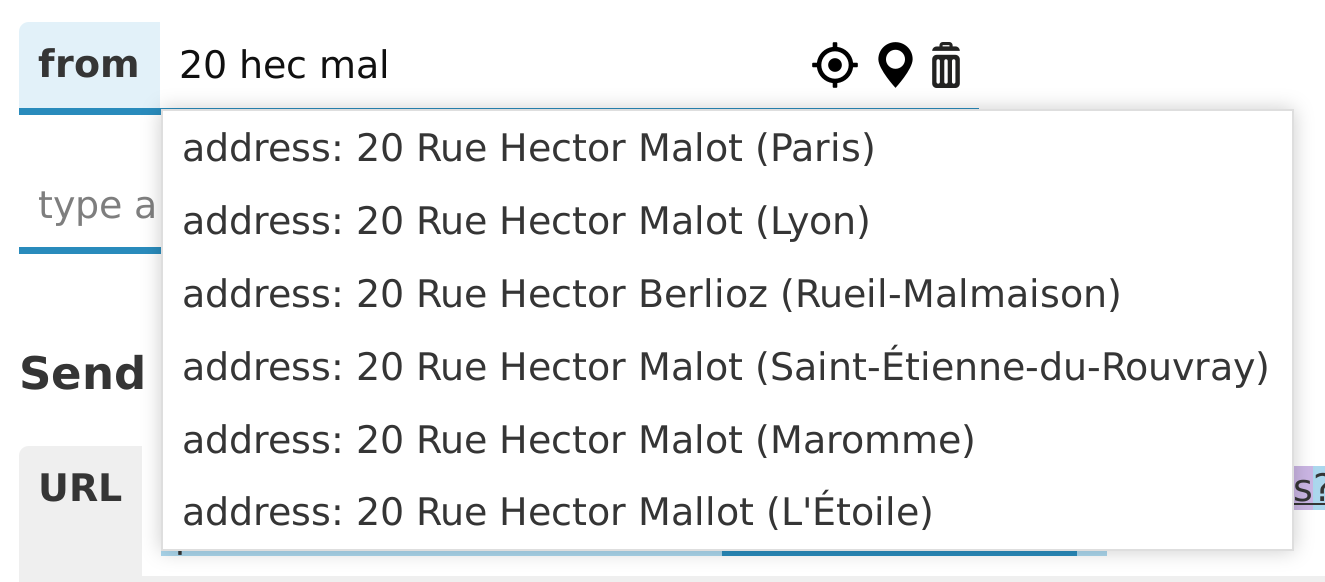
\includegraphics[width=\textwidth]{images/autocomplete-20-hec-mal}
      \end{block}
      \begin{block}{\strut 3 Place de la République (Paris)}
        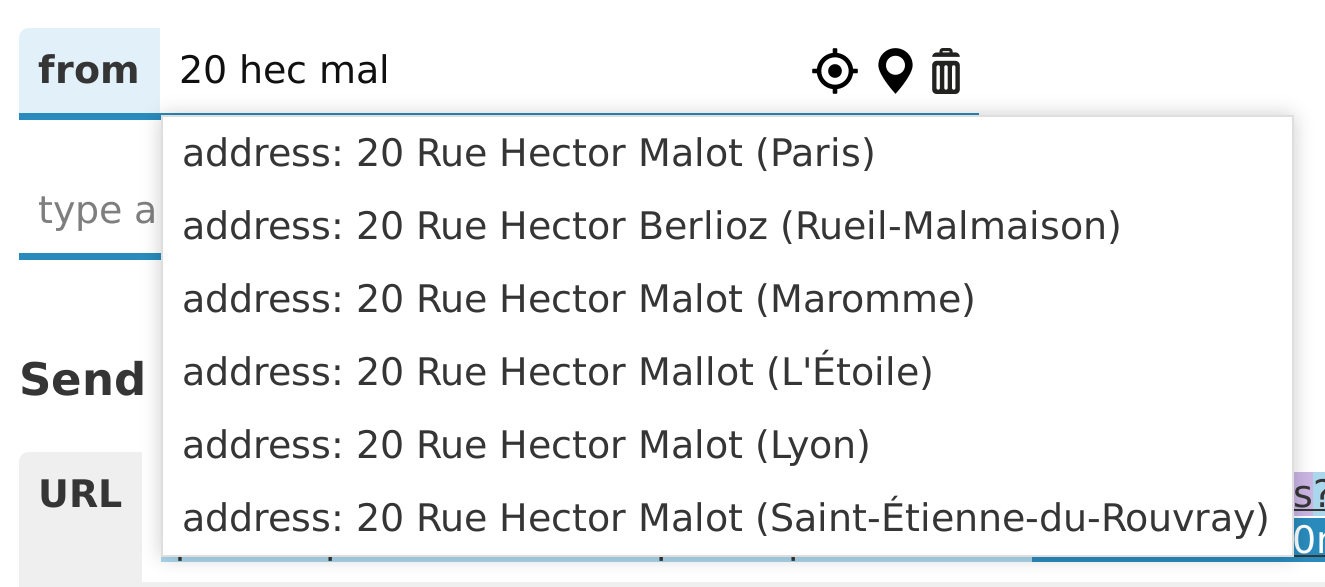
\includegraphics[width=\textwidth]{images/autocomplete-20-hec-mal-paris}
      \end{block}
    \end{column}
    \begin{column}{.5\linewidth}
      \begin{block}{\strut 3 Rue Lebrument (Rouen)}
        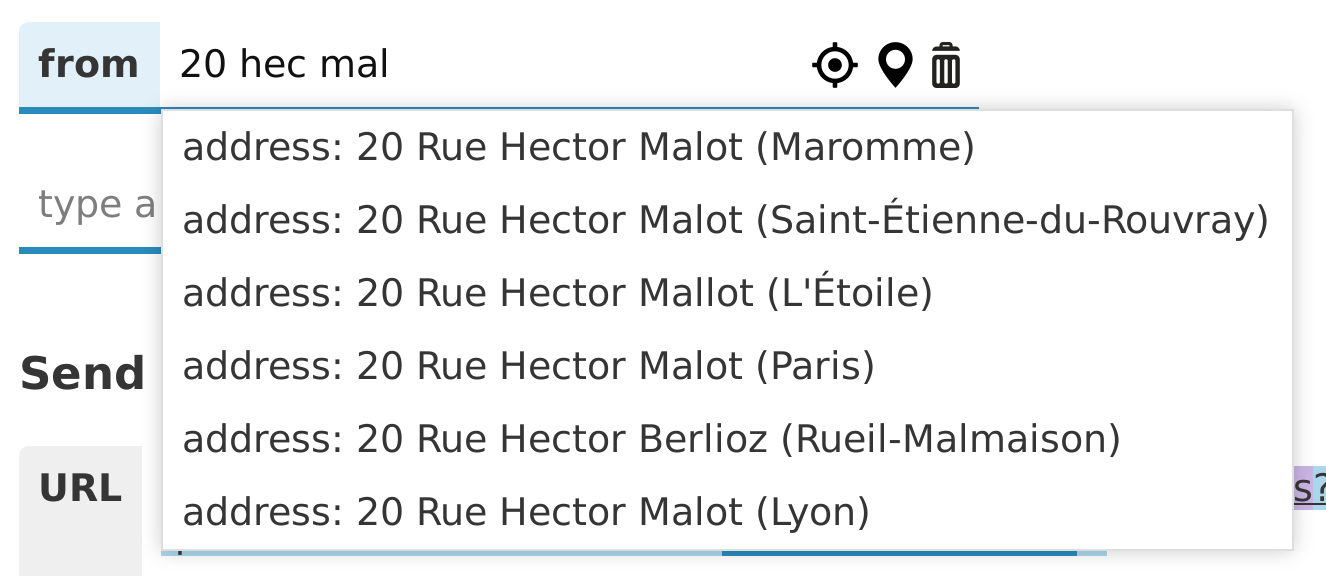
\includegraphics[width=\textwidth]{images/autocomplete-20-hec-mal-rouen}
      \end{block}
      \begin{block}{\strut 2 Rue de la République (Lyon)}
        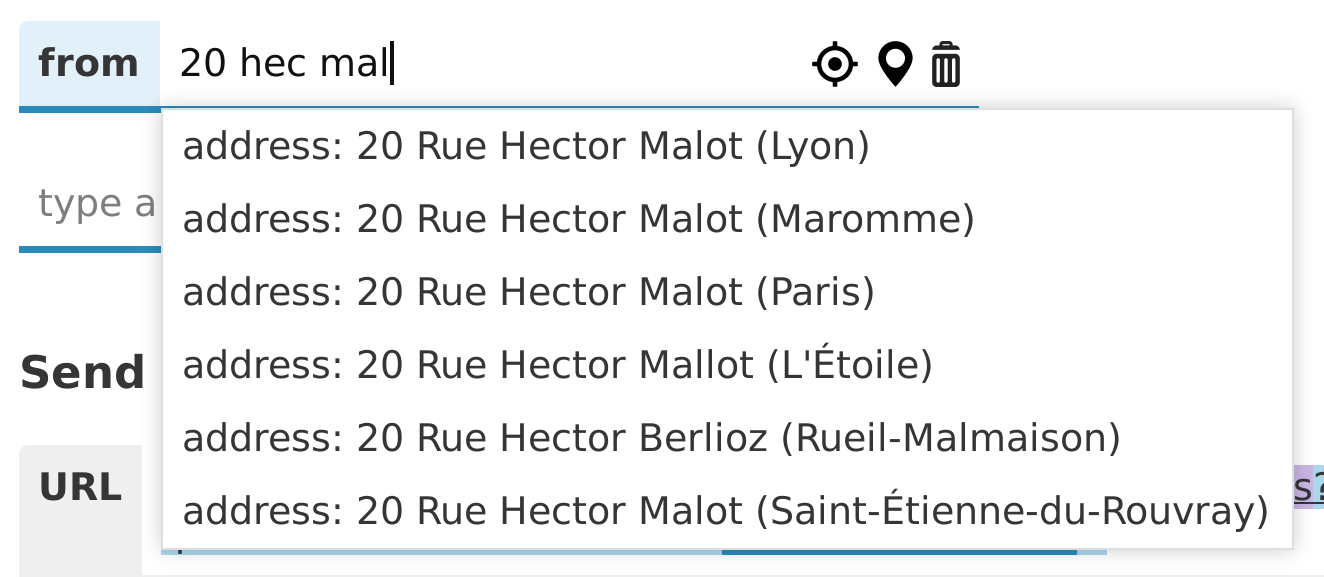
\includegraphics[width=\textwidth]{images/autocomplete-20-hec-mal-lyon}
      \end{block}
    \end{column}
  \end{columns}
\end{frame}

\begin{frame}
  \frametitle{Geolocalisation inversée}

  \centering
  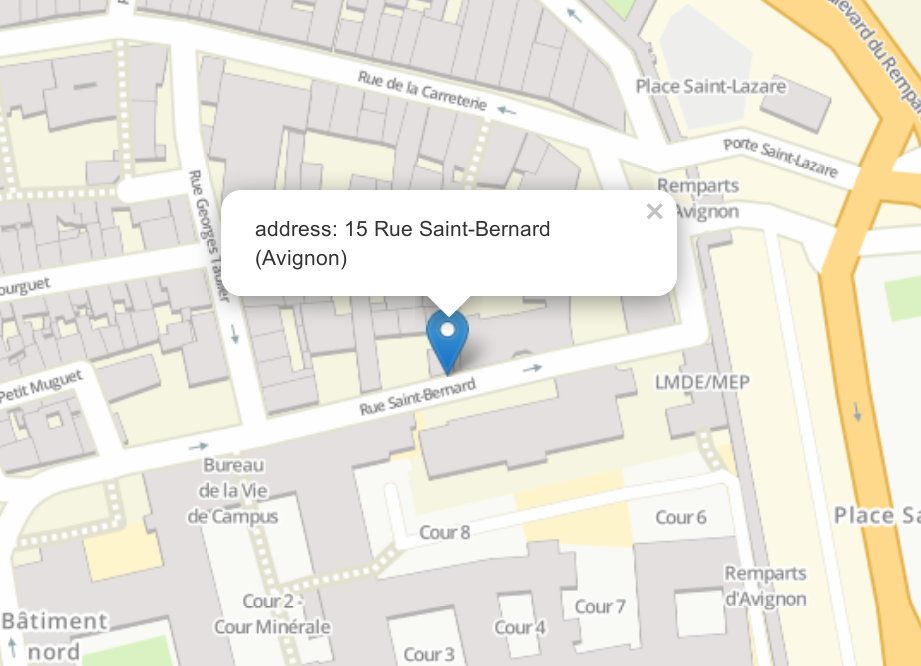
\includegraphics[width=.8\linewidth]{images/reverse-geocoding}
\end{frame}

\section{Retour d'expérience}

\begin{frame}
  \frametitle{OpenStreetMap}

  Les plus:
  \begin{itemize}
  \item bons contours géographiques pour les régions administratives
  \item corrections instantanées
  \item bonne qualité des rues
  \item communauté sympa et réactive
  \end{itemize}

  Les moins:
  \begin{itemize}
  \item complexité de modélisation (plusieurs moyens de modéliser la
    même chose, liens non implicite de la ville, codes postaux,
    contours géographiques...)
  \item problèmes de contributions (contours cassées, rues mal regroupées...)
  \item peu d'adresses
  \end{itemize}
\end{frame}

\begin{frame}
  \frametitle{BANO}

  Les plus:
  \begin{itemize}
  \item couverture quasi parfaite de la France
  \item corrections réalisables facilement
  \end{itemize}

  Les moins:
  \begin{itemize}
  \item pas d'évolution
  \item pas de stratégie de fusion BAN/BANO
  \end{itemize}
\end{frame}

\section{Technique}

\begin{frame}
  \frametitle{Technique}

  schema: data -> *2mimir -> base (mimir) -> bragi -> jormungandr
\end{frame}

\section{Conclusion}

\begin{frame}
  \frametitle{Conclusion}

  liens github, navitia.io, demo
\end{frame}

\begin{frame}
  \titlepage
\end{frame}

\end{document}
